\chapter{动能与道路安全}\label{ch:g9:kinetic-energy-safety}

自童年的发条玩具起，\omterm{def:g5:everyday-energy:energy}{能量}便是一个关于储存与形式的故事——
生动、有用，却没有数字。
现在，等待结束了。运动的\omterm{def:g5:everyday-energy:energy}{能量}有了它的公式，
\omterm{def:g5:everyday-energy:energy}{能量}有了它的\omterm{def:g6:measurement-in-science:measuring}{单位}，而这套运算竟关乎生死：
为什么\omterm{def:g7:motion-average-speed:formula}{速度}加倍的汽车，停下来要多花四倍的距离，
而一秒钟的分心要付出多少代价，
以米计。

\section{运动的能量}

\begin{definition}[焦耳]\label{def:g9:kinetic-energy-safety:joule}
\omterm{def:g5:everyday-energy:energy}{能量}——无论哪种形式——都以
\emph{焦耳}\index{焦耳}（\unit{J}）为\omterm{def:g6:measurement-in-science:measuring}{单位}度量，以纪念
那位证明热本身是一种\omterm{def:g5:everyday-energy:energy}{能量}形式的实验家。参照：
把这本书从地面举到书架上，约耗费几焦耳；
心脏每跳一次，约耗费一焦耳；
一块巧克力储存的食物\omterm{def:g5:everyday-energy:energy}{能量}达一百万焦耳。
\end{definition}

\begin{proposition}[动能]\label{prop:g9:kinetic-energy-safety:formula}
\omterm{def:g3:measuring-mass:mass}{质量}为 $m$（\omterm{def:g6:measurement-in-science:measuring}{单位}为\unit{kg}）、以\omterm{def:g7:motion-average-speed:formula}{速度} $v$（\omterm{def:g6:measurement-in-science:measuring}{单位}为
\unit{m/s}）运动的物体，因其运动而具有
\emph{动能}\index{动能}
\[
E_k = \frac{1}{2} \times m \times v^2 ,
\]
\omterm{def:g6:measurement-in-science:measuring}{单位}为\omterm{def:g9:kinetic-energy-safety:joule}{焦耳}。两个旋钮，幂次不同：\omterm{def:g3:measuring-mass:mass}{质量}加倍，
$E_k$ 也加倍——但\emph{\omterm{def:g7:motion-average-speed:formula}{速度}}加倍时，
\omterm{prop:g9:kinetic-energy-safety:formula}{动能}\emph{变为四倍}，因为\omterm{def:g7:motion-average-speed:formula}{速度}以平方的形式进入。
\omterm{def:g7:motion-average-speed:formula}{速度}才是危险的旋钮。
\end{proposition}

\begin{example}[初步计算]\label{ex:g9:kinetic-energy-safety:first}
\omterm{def:g3:measuring-mass:mass}{质量}为 \qty{0.45}{kg} 的足球，以 \qty{20}{m/s} 运动：$E_k = 0.5 \times
0.45 \times 20^2 = \qty{90}{J}$。\omterm{def:g3:measuring-mass:mass}{质量}为 \qty{60}{kg} 的短跑运动员，以
\qty{10}{m/s} 运动：$0.5 \times 60 \times 100 = \qty{3000}{J}$。\omterm{def:g3:measuring-mass:mass}{质量}为
\qty{1000}{kg} 的汽车，以 \qty{50}{km/h} 行驶——先换算\omterm{def:g6:measurement-in-science:measuring}{单位}：
$50 \div 3.6 \approx \qty{13.9}{m/s}$ --- $E_k = 0.5 \times
1000 \times 13.9^2 \approx \qty{9.7e4}{J}$：接近十万\omterm{def:g9:kinetic-energy-safety:joule}{焦耳}。同一辆车以
\qty{100}{km/h} 行驶时，\omterm{prop:g9:kinetic-energy-safety:formula}{动能}为前者的四倍，
即 \qty{3.9e5}{J}。公式的警告，
就写在这些数字里。
\end{example}

\begin{omfigure}
\begin{tikzpicture}
\begin{axis}[omaxis, width=10.2cm, height=6.0cm,
    xlabel={速度 $v$（\unit{km/h}）},
    ylabel={$E_k$（\unit{kJ}）},
    xtick={0,30,50,70,90,110,130}, ytick={0,100,200,300,400,500},
    ymin=0, ymax=560, xmin=0, xmax=140, samples=100]
  \addplot[very thick, omThm, domain=0:135]
    {0.5*1000*(x/3.6)^2/1000};
  \addplot[only marks, mark=*, omDef] coordinates
    {(50,96.5) (100,385.8)};
  \node[right, font=\small, omDef] at (axis cs:38,130)
    {\qty{50}{km/h}};
  \node[left, font=\small, omDef] at (axis cs:99,400)
    {\qty{100}{km/h}：四倍};
\end{axis}
\end{tikzpicture}

{\small 一吨重汽车的\omterm{prop:g9:kinetic-energy-safety:formula}{动能}随\omterm{def:g7:motion-average-speed:formula}{速度}的变化：它不是直线，
而是一条抛物线——公式中的平方，在此被画了出来。
\omterm{def:g7:motion-average-speed:formula}{速度}加倍，需要消散的\omterm{def:g5:everyday-energy:energy}{能量}便增至四倍。}
\end{omfigure}

\begin{example}[刹车把能量送往何处]\label{ex:g9:kinetic-energy-safety:brakes}
要使汽车停下，就必须把它全部的 $E_k$ 交给某物——
\omterm{def:g5:everyday-energy:energy}{能量}只会转移，绝不会消失，正如你童年时的链条所教导的那样。
刹车片的摩擦将其转化为\omterm{def:g5:heat-and-insulation:heat}{热量}：
下山之后，刹车盘会泛出琥珀色的光，而热刹车的焦味，
\emph{正是}\omterm{prop:g9:kinetic-energy-safety:formula}{动能}在退场。
在碰撞中，这种交接既剧烈又瞬间完成——\omterm{def:g5:everyday-energy:energy}{能量}流入扭曲的钢板。
下面每一个道路安全的数字，都是这笔账的结果：
$E_k$ 越大，它退场的过程就越长，或越惨烈。
\end{example}

\begin{omfigure}
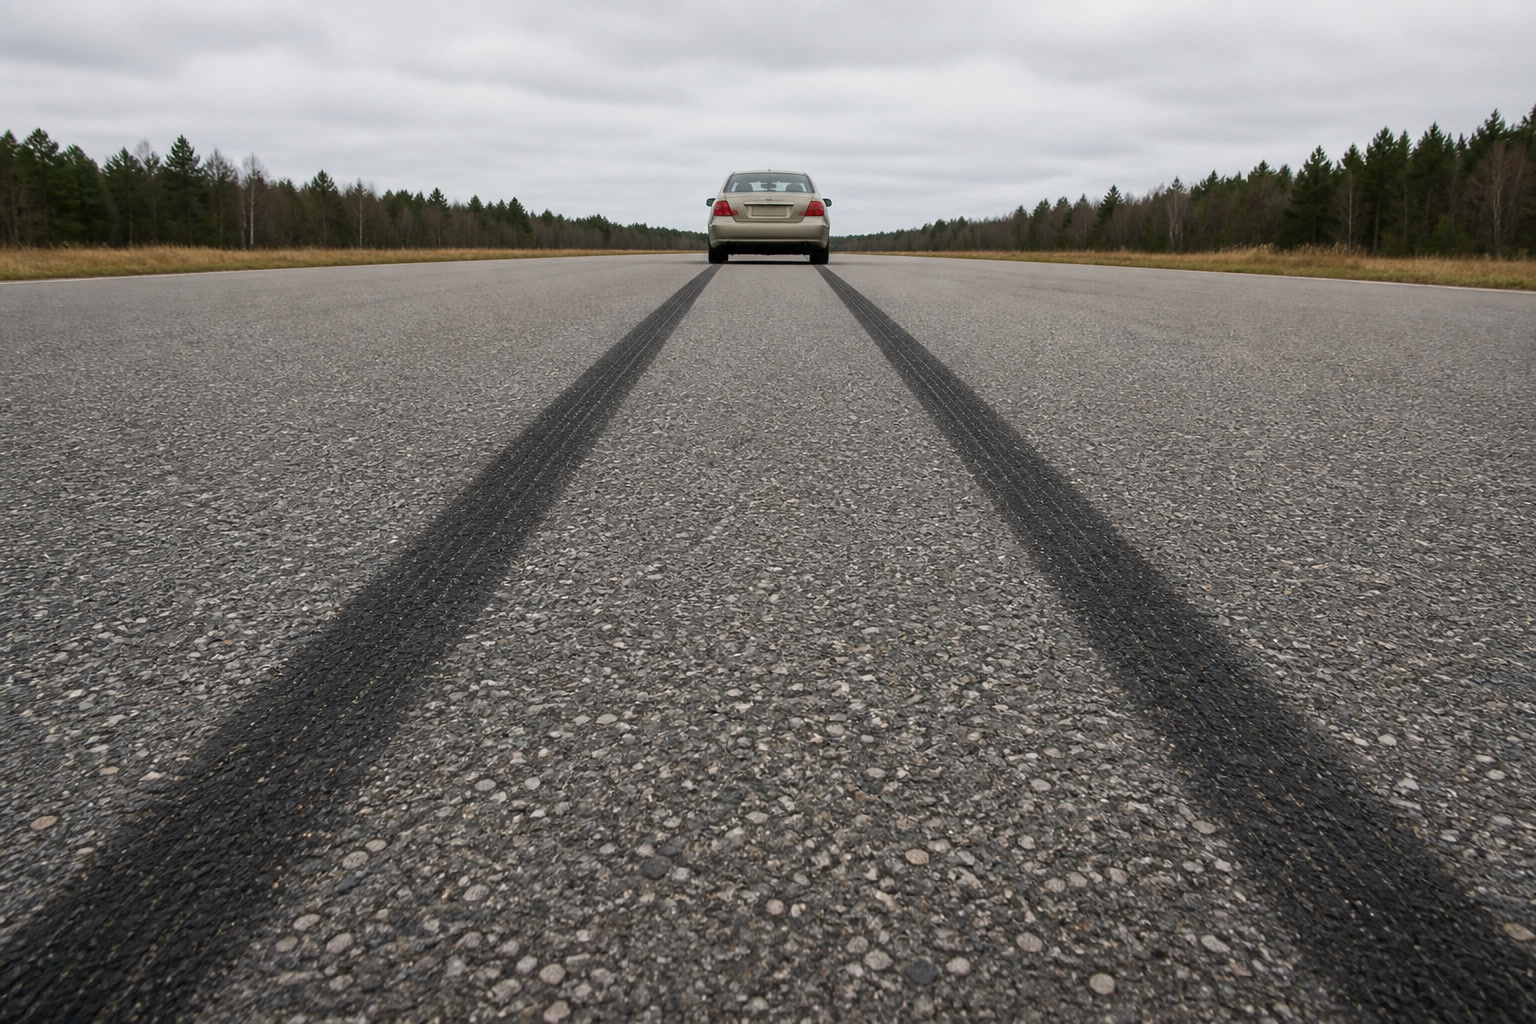
\includegraphics[width=0.55\linewidth]{images/book1/ai/g9-kinetic-skid-marks.jpg}

{\small \omterm{prop:g9:kinetic-energy-safety:formula}{动能}的去向：刹车与路面将其转化为\omterm{def:g5:heat-and-insulation:heat}{热量}，轮胎则在路面上留下了印记，作为凭证。}
\end{omfigure}

\section{停车距离}

\begin{proposition}[停车 = 反应 + 制动]\label{prop:g9:kinetic-energy-safety:stopping}
驾驶员发现险情后，
要经过两段路程才能停下：
\begin{enumerate}
  \item \emph{反应距离}\index{反应距离}：
        从大脑察觉险情到脚开始移动这段时间内所行驶的路程，
        \omterm{def:g7:motion-average-speed:formula}{速度}不变时约为一秒的行驶量，因此这段距离
        与 $v$ \emph{成正比}增长；
  \item \emph{制动距离}\index{制动距离}：
        刹车使\omterm{prop:g9:kinetic-energy-safety:formula}{动能}退场所需的路程——
        由于 $E_k$ 含有 $v^2$，这段距离随\omterm{def:g7:motion-average-speed:formula}{速度}的
        \emph{平方}增长：\omterm{def:g7:motion-average-speed:formula}{速度}加倍，
        \omterm{prop:g9:kinetic-energy-safety:stopping}{制动距离}便增至四倍。
\end{enumerate}
两者之和，即\emph{停车距离}，
正是那个追球的孩子所遭遇的数字。
\end{proposition}

\begin{example}[每位驾驶员都应掌握的表格]\label{ex:g9:kinetic-energy-safety:table}
干燥路面，驾驶员警觉（反应时间一秒，刹车性能良好）：
\begin{center}
\begin{tabular}{l|c|c|c}
\omterm{def:g7:motion-average-speed:formula}{速度} & \omterm{prop:g9:kinetic-energy-safety:stopping}{反应距离} & \omterm{prop:g9:kinetic-energy-safety:stopping}{制动距离} & 停车距离 \\
\hline
\qty{50}{km/h} & \qty{14}{m} & \qty{13}{m} & \qty{27}{m} \\
\qty{90}{km/h} & \qty{25}{m} & \qty{40}{m} & \qty{65}{m} \\
\qty{130}{km/h} & \qty{36}{m} & \qty{85}{m} & \qty{121}{m}
\end{tabular}
\end{center}
请仔细读两遍。城市车速下，停车距离约为一个半公交车长；
高速公路车速下，约为一条标准跑道的全长再加五分之一。
比例也印证了两条规律：\omterm{prop:g9:kinetic-energy-safety:stopping}{反应距离}随 $v$ 增长，
\omterm{prop:g9:kinetic-energy-safety:stopping}{制动距离}随 $v^2$ 增长——高速行驶时，\omterm{prop:g9:kinetic-energy-safety:stopping}{制动距离}
占去了总距离的大部分。
\end{example}

\begin{method}[估算停车距离]\label{met:g9:kinetic-energy-safety:estimate}
\begin{enumerate}
  \item 将\omterm{def:g7:motion-average-speed:formula}{速度}换算为 \unit{m/s}（把 \unit{km/h}
        数值除以 $3.6$）；
  \item \omterm{prop:g9:kinetic-energy-safety:stopping}{反应距离}：一秒内行驶的距离——即
        \unit{m/s} 的数值本身，\omterm{def:g6:measurement-in-science:measuring}{单位}为米；
  \item \omterm{prop:g9:kinetic-energy-safety:stopping}{制动距离}：以已知参照值按平方比例换算——
        即从 \qty{50}{km/h} 时的 \qty{13}{m} 出发，乘以
        $(v/50)^2$；
  \item 相加，并与前方道路实际可供的
        通行距离相比较。
\end{enumerate}
路面潮湿时，\omterm{prop:g9:kinetic-energy-safety:stopping}{制动距离}会加倍；疲劳或分心的
驾驶员会使反应时间延长至接近两秒——
请用真实的输入值重新计算总和。
\end{method}

\begin{example}[一瞥的代价]\label{ex:g9:kinetic-energy-safety:glance}
在 \qty{90}{km/h} 时用两秒钟瞥一眼手机：汽车
行驶了 $2 \times 25 = \qty{50}{m}$——约为半个足球场的长度
——尚未等到任何一秒的反应时间开始，就已盲目驶过。
在城市车速下，同样一瞥会盲目消耗 \qty{28}{m}：
驶过路口，驶过校门。
汽车中最危险的部件，是本节中任何公式都无法
度量的：驾驶员的注意力。
\end{example}

\begin{remark}[安全带、安全气囊与头盔]\label{rem:g9:kinetic-energy-safety:belts}
碰撞时，汽车在约一米的车身压溃中停下——但
未系安全带的乘客仍以原速前行（上一章那句
平静的话，此刻残酷地应验），直到被
途中所遇之物挡住：仪表盘、挡风玻璃、路面。安全带与
安全气囊则在更长的距离和时间内让身体停下，
使其\omterm{prop:g9:kinetic-energy-safety:formula}{动能}温和地消散，而非一次性完成；
骑车人的头盔对颅骨
内那些无法替代的东西起到同样作用，其可压碎的泡沫
为之争取了数\omterm{def:g2:measuring-length:units}{厘米}的温和\omterm{prop:g9:kinetic-energy-safety:stopping}{制动距离}。它们都不能使你的
$E_k$ 减少哪怕一\omterm{def:g9:kinetic-energy-safety:joule}{焦耳}——它们只是让其消散变得文明。
\end{remark}

\section{练习}

\begin{exercise}[$\star$]\label{exo:g9:kinetic-energy-safety:1}
写出\omterm{def:g5:everyday-energy:energy}{能量}的\omterm{def:g6:measurement-in-science:measuring}{单位}及其两个参照值，并写出
\omterm{prop:g9:kinetic-energy-safety:formula}{动能}公式以及公式中各量的\omterm{def:g6:measurement-in-science:measuring}{单位}。
\end{exercise}

\begin{exercise}[$\star$]\label{exo:g9:kinetic-energy-safety:2}
计算 $E_k$：\omterm{def:g3:measuring-mass:mass}{质量}为 \qty{2}{kg}、\omterm{def:g7:motion-average-speed:formula}{速度}为 \qty{10}{m/s} 的野兔；
\omterm{def:g3:measuring-mass:mass}{质量}为 \qty{80}{kg}、\omterm{def:g7:motion-average-speed:formula}{速度}为 \qty{5}{m/s} 的橄榄球运动员。
\end{exercise}

\begin{exercise}[$\star$]\label{exo:g9:kinetic-energy-safety:3}
哪种做法能使汽车的 $E_k$ 增加得更多：加上相当于
其\omterm{def:g3:measuring-mass:mass}{质量}一半的货物，还是把\omterm{def:g7:motion-average-speed:formula}{速度}提高一半？请写出两种情形各自的因子。
\end{exercise}

\begin{exercise}[$\star$]\label{exo:g9:kinetic-energy-safety:4}
说出停车距离的两个组成部分，及其
增长规律：一段正比于\omterm{def:g7:motion-average-speed:formula}{速度}，另一段正比于\omterm{def:g7:motion-average-speed:formula}{速度}的平方。
\end{exercise}

\begin{exercise}[$\star$]\label{exo:g9:kinetic-energy-safety:5}
根据驾驶员表格，停车距离中\omterm{prop:g9:kinetic-energy-safety:stopping}{制动距离}所占的
比例在 \qty{50}{km/h} 时是多少——在 \qty{130}{km/h} 时又是多少？
这一比例发生了什么变化？
\end{exercise}

\begin{exercise}[$\star$]\label{exo:g9:kinetic-energy-safety:6}
制动时，汽车的\omterm{prop:g9:kinetic-energy-safety:formula}{动能}去了哪里？请举出你能闻到的气味
和看到的灼热之光——以及那条禁止\omterm{prop:g9:kinetic-energy-safety:formula}{动能}凭空消失的
儿时就学过的定律。
\end{exercise}

\begin{exercise}[$\star$]\label{exo:g9:kinetic-energy-safety:7}
计算\omterm{def:g7:motion-average-speed:formula}{速度}分别为 \qty{36}{km/h}、
\qty{72}{km/h} 和 \qty{108}{km/h} 时的\omterm{prop:g9:kinetic-energy-safety:stopping}{反应距离}（取警觉的一秒）。
这些结果呈现出怎样的简单规律？
\end{exercise}

\begin{exercise}[$\star$]\label{exo:g9:kinetic-energy-safety:8}
为什么安全带不能减少你的\omterm{prop:g9:kinetic-energy-safety:formula}{动能}——它
转而使什么的消散变得文明？
\end{exercise}

\begin{exercise}[$\star\star$]\label{exo:g9:kinetic-energy-safety:9}
一辆滑板车在 \qty{30}{km/h} 时的\omterm{prop:g9:kinetic-energy-safety:stopping}{制动距离}为 \qty{8}{m}。
试估算其在 \qty{60}{km/h} 和 \qty{90}{km/h} 时的\omterm{prop:g9:kinetic-energy-safety:stopping}{制动距离}，并
说明你所依据的换算规律。
\end{exercise}

\begin{exercise}[$\star\star$]\label{exo:g9:kinetic-energy-safety:10}
各地市镇议会把学校周边路段的限速从 \qty{50}{} 降至
\qty{30}{km/h}。比较两种情况下的停车距离（参照：
在 $50$ 时\omterm{prop:g9:kinetic-energy-safety:stopping}{制动距离}为 \qty{13}{m}，反应时间取一秒）——并
比较两者的\omterm{prop:g9:kinetic-energy-safety:formula}{动能}。你认为哪一种比较
在海报上更有说服力？
\end{exercise}

\begin{exercise}[$\star\star$]\label{exo:g9:kinetic-energy-safety:11}
降雨使\omterm{prop:g9:kinetic-energy-safety:stopping}{制动距离}加倍。请重新计算驾驶员表格中
潮湿路面在 $50$ 和 \qty{90}{km/h} 时的停车距离一栏——
你将哪一部分加倍了，哪一部分没有，为什么？
\end{exercise}

\begin{exercise}[$\star\star\star$]\label{exo:g9:kinetic-energy-safety:12}
一辆\omterm{def:g3:measuring-mass:mass}{质量}为 \qty{20000}{kg} 的卡车以 \qty{90}{km/h} 的\omterm{def:g7:motion-average-speed:formula}{速度}行驶。计算
其 $E_k$（用科学记数法表示）；求出一辆\omterm{def:g3:measuring-mass:mass}{质量}为
\qty{1000}{kg} 的汽车获得相同\omterm{prop:g9:kinetic-energy-safety:formula}{动能}时的\omterm{def:g7:motion-average-speed:formula}{速度}（令两式
相等——代数运算留给你今年完成）；并
总结为何山区公路上设有失控卡车避险车道，
而汽车却无此类车道。
\end{exercise}

\section{问题：安全宣传活动}

\begin{problem}[{周末问题——班级设计镇上的
道路安全宣传活动；海报用公式检验；
市长的难题}]\label{pb:g9:kinetic-energy-safety:1}
镇上委托开展一项宣传活动，条件只有一个：
每张海报上的每个数字都必须经得起物理审核。
班级动手计算。（已知条件：反应时间为一秒；\omterm{prop:g9:kinetic-energy-safety:stopping}{制动
距离}在 \qty{50}{km/h} 下为 \qty{13}{m}，按平方关系换算；汽车
\omterm{def:g3:measuring-mass:mass}{质量}为 \qty{1000}{kg}。）

\medskip\noindent\textbf{第一部分——海报一：“50 而非
60”。}
\begin{enumerate}
  \item 以 \unit{m/s} 为\omterm{def:g6:measurement-in-science:measuring}{单位}，计算两个\omterm{def:g7:motion-average-speed:formula}{速度}（保留一位小数）。
  \item 两种\omterm{def:g7:motion-average-speed:formula}{速度}下的\omterm{prop:g9:kinetic-energy-safety:stopping}{反应距离}各是多少？
  \item 两种\omterm{def:g7:motion-average-speed:formula}{速度}下的\omterm{prop:g9:kinetic-energy-safety:stopping}{制动距离}各是多少（按已知条件换算）？
  \item 海报标题：“\omterm{def:g7:motion-average-speed:formula}{速度}每增加十个\omterm{def:g6:measurement-in-science:measuring}{单位}，
        停车距离多出多少米？”请填写
        该数字。
\end{enumerate}

\medskip\noindent\textbf{第二部分——海报二：“\omterm{def:g7:motion-average-speed:formula}{速度}之
墙”。}
设计图以下落高度表示碰撞\omterm{def:g5:everyday-energy:energy}{能量}：\omterm{def:g7:motion-average-speed:formula}{速度}为
$v$ 的碰撞“相当于”从某一高度下落，
即下落所获\omterm{def:g5:everyday-energy:energy}{能量}与之相同的那一高度。
\begin{enumerate}[resume]
  \item 计算汽车在 \qty{50}{km/h} 时的 $E_k$（数据取自
        第一部分），以及 \qty{90}{km/h} 时的\omterm{prop:g9:kinetic-energy-safety:formula}{动能}。
  \item 美工需要高度数据：对本车而言，从 \qty{1}{m} 高处下落
        约获得 \qty{9.8}{kJ} 的\omterm{def:g5:everyday-energy:energy}{能量}（$m g h$ 为
        下一章的公式，此处提前借用）。两种碰撞\omterm{def:g5:everyday-energy:energy}{能量}
        分别对应多高的下落高度？
        （请做除法，结果取整到米。）
  \item 哪些日常建筑的高度与之相当？拟定
        海报上的文案。
  \item 市长提出异议：“没有人会直接撞墙；
        汽车会变形，安全带会拉住人。”请在承认其
        观点的同时为海报的物理内容辩护——吸能区与
        安全带改变了什么，
        又有哪些数值并未改变？
\end{enumerate}

\medskip\noindent\textbf{第三部分——海报三：“一
秒”。}
\begin{enumerate}[resume]
  \item 以 \qty{90}{km/h} 行驶时，
        分心一秒在开始制动前要耗去多少米？再看
        两秒钟的手机一瞥呢？
  \item 疲劳驾驶版本：反应时间延长到两
        秒。重新计算
        \qty{90}{km/h} 下的完整停车距离，并与清醒驾驶员的
        \qty{65}{m} 作比较。
  \item 一位持怀疑态度的议员说：“与那些很大的制动数字相比，
        一秒钟应该无足轻重吧。”他在哪种\omterm{def:g7:motion-average-speed:formula}{速度}下错得最离谱——
        低速还是高速？（比较两项距离的增长规律。）
        的两个分量的增长规律。）
  \item 定稿宣传活动：三张海报的底部各写一行字，
        每张一行，各配一条公式，
        用通俗的语言表述。
\end{enumerate}
\end{problem}
